\section{SYS\_08 -- Falco}

\subsection{Introduzione a Falco e sicurezza runtime}

\subsubsection{Sicurezza runtime e monitoraggio nei cluster}



La \emph{runtime security} si occupa di monitorare e proteggere il comportamento dei sistemi e delle applicazioni durante la loro esecuzione. Nelle architetture moderne, in particolare quelle basate su container e orchestratori come Kubernetes, questo tipo di monitoraggio è fondamentale per individuare attività sospette, violazioni delle policy e compromissioni che non sono rilevabili nella fase di build o di configurazione.

In un cluster Kubernetes è necessario osservare ciò che accade senza introdurre modifiche alle applicazioni né degradare le prestazioni. Una soluzione diffusa è il pattern \emph{sidecar}, che affianca a ogni container applicativo un container di monitoraggio. Questo approccio fornisce visibilità locale sul pod, ma non consente una visione completa del sistema.

Un’alternativa più profonda è il monitoraggio a livello di kernel, che permette di osservare direttamente le interazioni tra applicazioni e sistema operativo, fornendo una visibilità globale e indipendente dalla tecnologia applicativa utilizzata.

\begin{figure}[H]
\centering
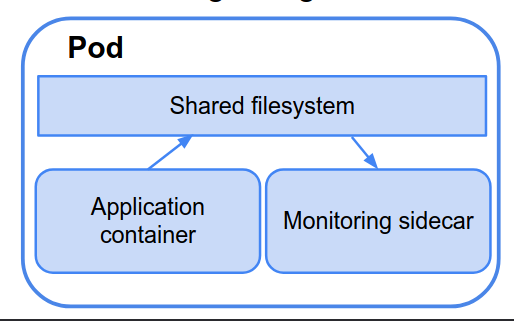
\includegraphics[width=0.7\textwidth]{immagini/SYS_08/sidecar.png}
\caption{Pattern sidecar in Kubernetes: il container applicativo e il container di monitoraggio condividono lo stesso filesystem all’interno del pod, consentendo l’osservazione del comportamento dell’applicazione senza modificarne il codice.}

\end{figure}

\subsubsection{Syscall e monitoraggio del kernel}

Le \emph{system call} rappresentano il principale punto di contatto tra lo \emph{user space}, in cui girano le applicazioni, e il kernel, che gestisce risorse fondamentali come file system, rete e memoria. Operazioni comuni come \texttt{open()}, \texttt{read()}, \texttt{write()} o \texttt{fork()} passano necessariamente attraverso una syscall.

Monitorare le syscalls consente di comprendere in modo preciso il comportamento di un sistema, poiché ogni interazione significativa con il kernel viene esplicitata. Tuttavia, esportare tutte le syscalls verso lo user space non è sostenibile: un sistema moderno può generare fino a milioni di syscalls al secondo.

Inoltre, per interpretare correttamente un evento è necessario arricchirlo con informazioni di contesto, come l’utente, il processo, il container o il namespace di appartenenza. Questo richiede l’integrazione con runtime container come Docker o containerd, ma tali interrogazioni possono introdurre latenza e ridurre l’efficacia del monitoraggio in tempo reale.

\subsubsection{Falco come sistema di rilevamento runtime}

Falco è un motore open-source di \emph{runtime threat detection} progettato per monitorare le syscalls in tempo reale su sistemi Linux. L’integrazione diretta con il kernel consente a Falco di intercettare eventi legati a operazioni sensibili, come accessi a file critici, modifiche ai permessi o tentativi di escalation dei privilegi.

Il punto di forza di Falco è il suo \emph{motore di regole}, basato su regole dichiarative in formato YAML, che descrivono comportamenti sospetti o vietati. Gli eventi raccolti vengono arricchiti con metadati contestuali (utente, processo, container), consentendo una rilevazione accurata anche in ambienti containerizzati.

Falco fornisce quindi una visibilità completa a livello di sistema, monitorando tutti i processi e i container in esecuzione e generando alert in tempo reale quando viene rilevato un comportamento anomalo.

\subsection{Architettura e funzionamento di Falco}

\subsubsection{Componenti principali}

Falco si basa su due componenti fondamentali:
\begin{itemize}
    \item i \textbf{driver di monitoraggio}, che catturano gli eventi a livello di kernel;
    \item il \textbf{motore di regole}, che analizza gli eventi e genera gli alert.
\end{itemize}

I driver possono essere implementati come moduli kernel tradizionali oppure tramite \emph{probe eBPF}. Questi ultimi rappresentano l’approccio più moderno e leggero, e sono particolarmente adatti a sistemi containerizzati e ambienti cloud-native.

\begin{figure}[H]
\centering
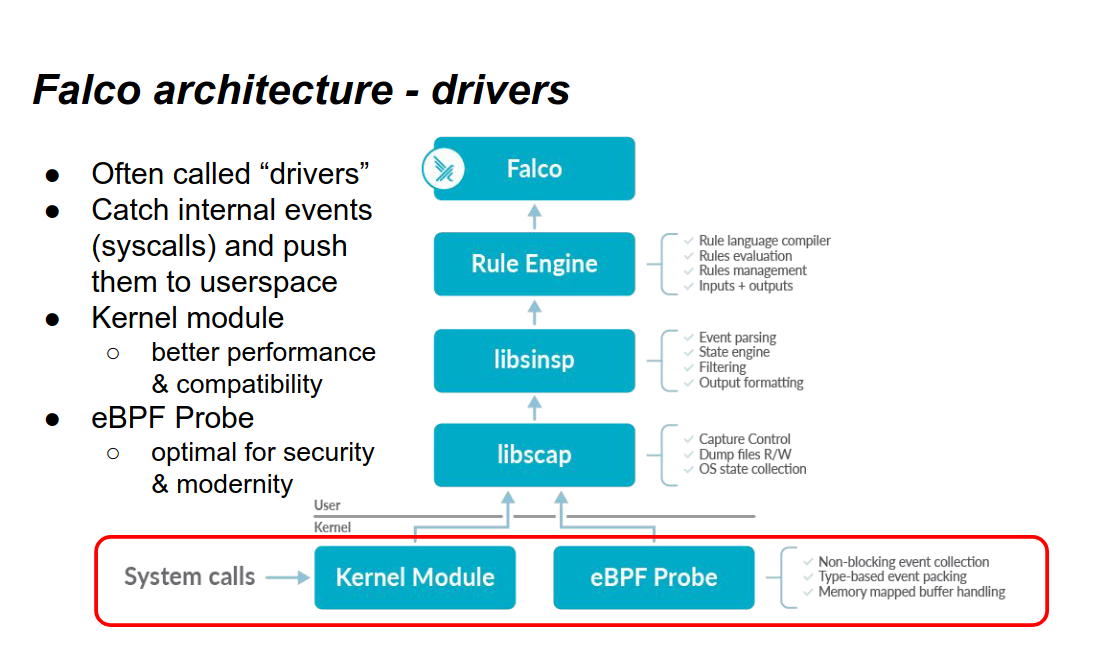
\includegraphics[width=0.8\textwidth]{immagini/SYS_08/architecture_driver.png}
\caption{Architettura di Falco: i driver (modulo kernel o probe eBPF) intercettano le system call nel kernel e inoltrano gli eventi allo user space, dove vengono elaborati dalle librerie di cattura e dal motore di regole per il rilevamento delle minacce.}
\end{figure}


\paragraph{Interazione kernel--user space}


Quando una syscall viene invocata, il driver intercetta l’evento e lo inserisce in un \emph{ring buffer}. Ogni CPU dispone del proprio buffer, riducendo la contesa e migliorando la scalabilità. Gli eventi vengono poi letti dallo user space tramite il dispositivo \texttt{/dev/falco}.

Le \emph{mappe eBPF} sono utilizzate per la gestione di dati a bassa latenza e per la comunicazione di informazioni di controllo tra kernel e user space.
\begin{figure}[H]
\centering
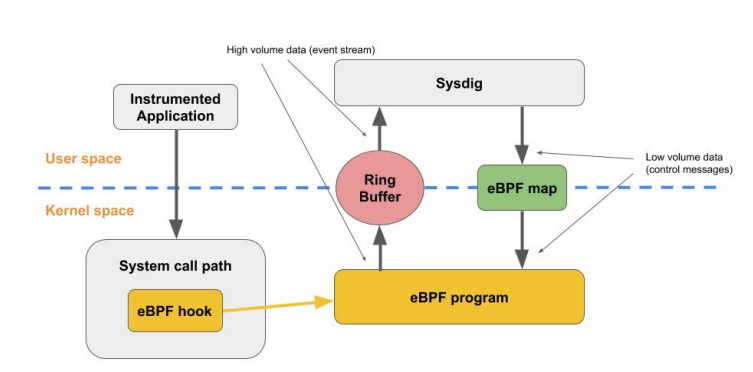
\includegraphics[width=0.8\textwidth]{immagini/SYS_08/maps.png}
\caption{Interazione tra kernel e user space tramite eBPF: gli eventi ad alto volume generati dalle system call vengono trasferiti tramite ring buffer, mentre le mappe eBPF sono utilizzate per lo scambio di dati di controllo a bassa latenza.}

\end{figure}




\subsection{Gestione degli eventi e performance}

Il monitoraggio continuo delle syscalls comporta un elevato volume di eventi. Per limitare l’overhead, Falco adotta diverse strategie:
\begin{itemize}
    \item buffering in memoria tramite ring buffer;
    \item filtraggio anticipato degli eventi;
    \item utilizzo di eBPF per ridurre il costo di intercettazione.
\end{itemize}

\begin{figure}[H]
\centering
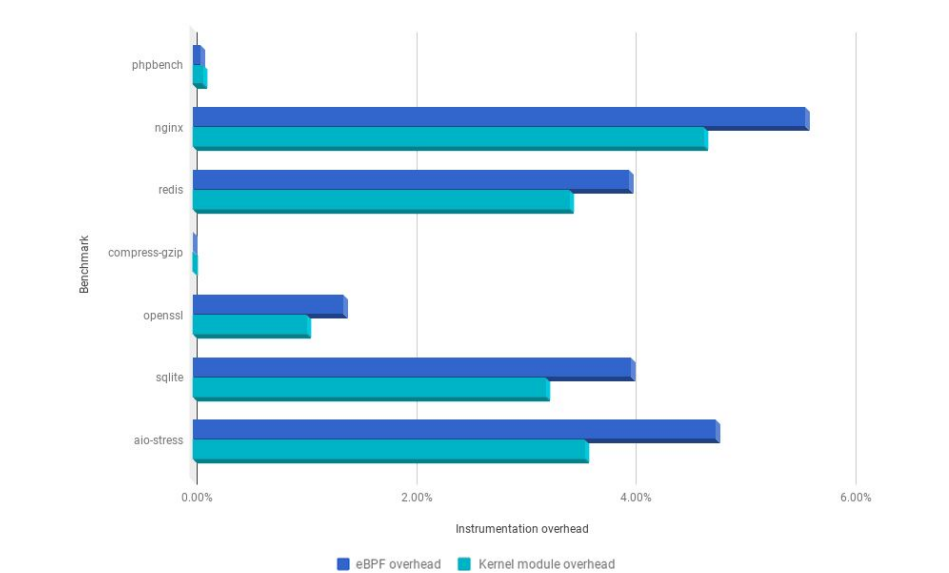
\includegraphics[width=0.8\textwidth]{immagini/SYS_08/ebpf.png}
\caption{eBPF Probe Overhead}
\end{figure}

Queste tecniche permettono a Falco di operare in tempo reale anche in sistemi ad alta intensità di eventi.

\subsection{Regole di Falco}

Le regole di Falco sono definite in formato YAML e descrivono i comportamenti che devono essere considerati sospetti durante l’esecuzione del sistema. Ogni regola specifica le condizioni in base alle quali un evento viene rilevato e il tipo di segnalazione da generare.

Una regola Falco è composta dai seguenti elementi fondamentali:
\begin{itemize}
    \item \textbf{rule}: nome identificativo della regola, utilizzato per riferirsi ad essa nei log e negli alert;
    \item \textbf{desc}: descrizione testuale del comportamento monitorato, utile a comprendere il significato della regola;
    \item \textbf{condition}: espressione logica che definisce le condizioni di attivazione della regola, basata sugli eventi di sistema (ad esempio system call, file descriptor, processo o utente);
    \item \textbf{output}: messaggio generato quando la regola viene attivata, che può includere variabili dinamiche per riportare i dettagli dell’evento rilevato;
    \item \textbf{priority}: livello di severità dell’alert (ad esempio \texttt{DEBUG}, \texttt{INFO}, \texttt{WARNING}, \texttt{ERROR});
    \item \textbf{tags}: insieme di etichette utilizzate per classificare la regola in base al dominio di sicurezza (filesystem, network, authentication, ecc.).
\end{itemize}

Per facilitare la scrittura e la manutenzione delle regole, Falco mette a disposizione costrutti riutilizzabili:
\begin{itemize}
    \item \textbf{macros}, che permettono di definire condizioni comuni riutilizzabili in più regole;
    \item \textbf{lists}, utilizzate per definire insiemi di valori (ad esempio file o indirizzi IP) da richiamare nelle condizioni;
    \item \textbf{template}, che consentono di standardizzare la formattazione degli output e ridurre la duplicazione.
\end{itemize}

\begin{figure}[H]
\centering
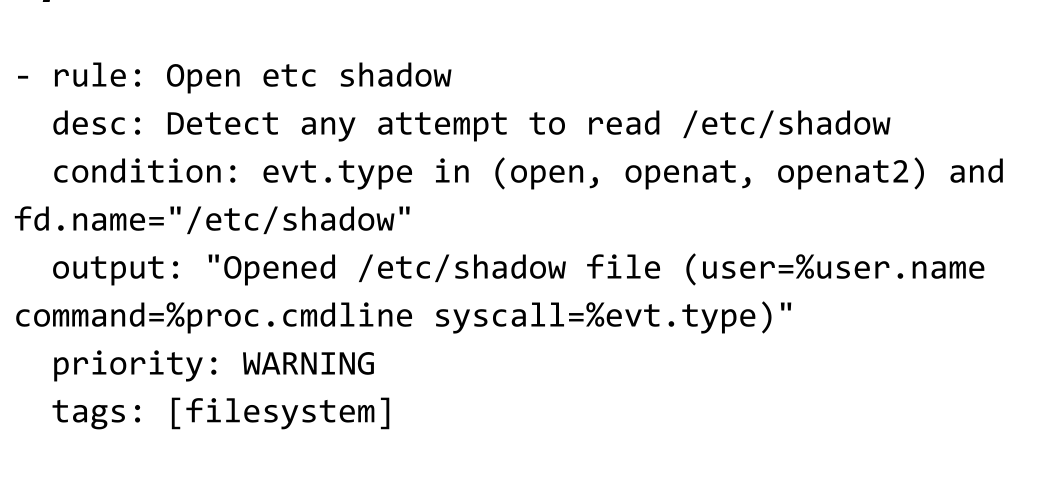
\includegraphics[width=0.8\textwidth]{immagini/SYS_08/rules.png}
\caption{Esempio di regola Falco per il rilevamento di tentativi di accesso al file sensibile \texttt{/etc/shadow}, basata sull’intercettazione delle system call di apertura dei file.}

\end{figure}


\subsection{Monitoraggio di rete e integrazione}

Oltre al monitoraggio delle operazioni su file e processi, Falco consente di osservare anche il comportamento di rete del sistema a runtime. Attraverso l’analisi delle system call di rete, Falco è in grado di rilevare connessioni in ingresso o in uscita che violano le policy di sicurezza, come comunicazioni verso indirizzi IP non autorizzati o endpoint inattesi.

Questo tipo di monitoraggio è particolarmente rilevante in ambienti containerizzati e microservizi, dove una connessione anomala può indicare attività di esfiltrazione dei dati, compromissione di un container o comunicazioni con server di comando e controllo (C\&C). Le regole possono includere informazioni di contesto, come processo, container e namespace, permettendo una rilevazione più accurata e riducendo i falsi positivi.

\begin{figure}[H]
\centering
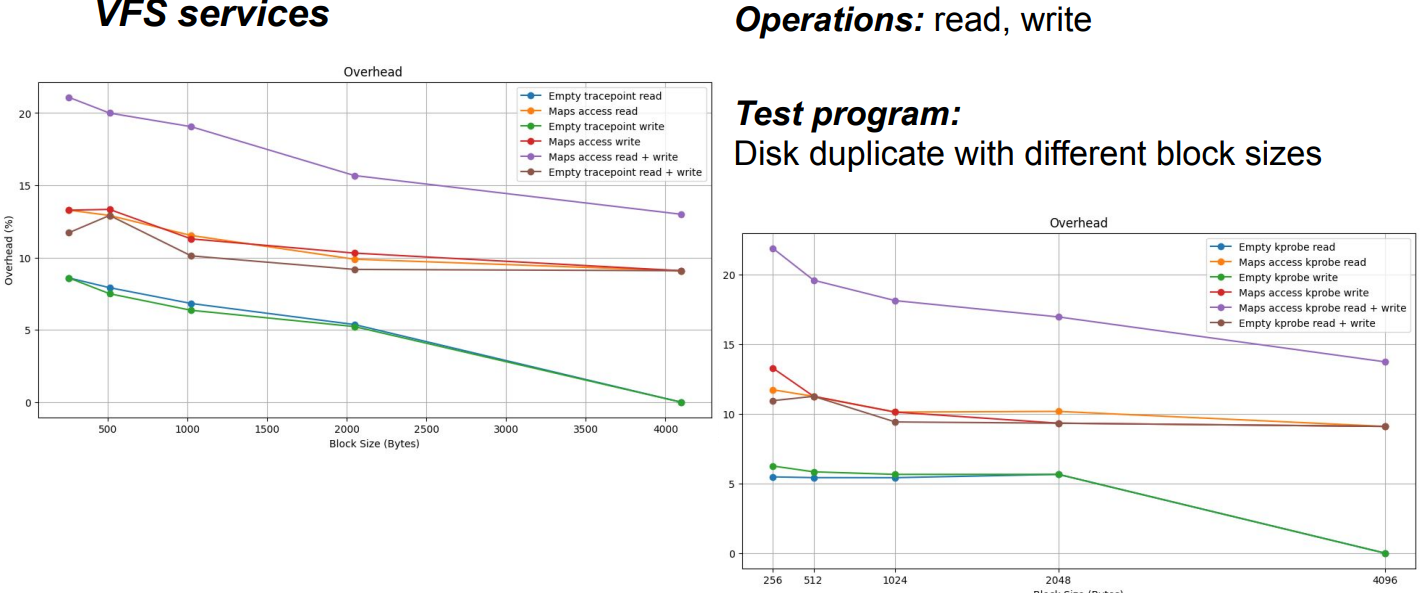
\includegraphics[width=0.8\textwidth]{immagini/SYS_08/runtime.png}
\caption{Costi runtime dei servizi di sistema durante il monitoraggio continuo}
\end{figure}

Gli eventi rilevati da Falco possono essere esportati in tempo reale verso sistemi esterni utilizzando formati strutturati come JSON o protocolli di comunicazione come gRPC. Questi meccanismi consentono di separare il motore di rilevamento dalla fase di analisi e risposta, favorendo un’architettura modulare e scalabile.

L’esportazione in formato \textbf{JSON} offre un’elevata interoperabilità: gli eventi possono essere facilmente consumati da sistemi di logging, SIEM o pipeline di elaborazione, risultando particolarmente adatta a integrazioni semplici e a scenari di analisi asincrona.

L’utilizzo di \textbf{gRPC}, invece, è pensato per integrazioni ad alte prestazioni e in tempo reale. Grazie alla comunicazione binaria e allo streaming degli eventi, gRPC consente una latenza ridotta e un uso più efficiente delle risorse, rendendolo adatto a sistemi di risposta automatizzata o a integrazioni dirette con IDS/IPS.

In questo modo Falco può essere integrato in un ecosistema di sicurezza più ampio, in cui gli eventi di sicurezza vengono non solo visualizzati, ma anche correlati e utilizzati per attivare contromisure automatiche.
\subsection{Limiti e considerazioni operative}

\begin{figure}[H]
\centering
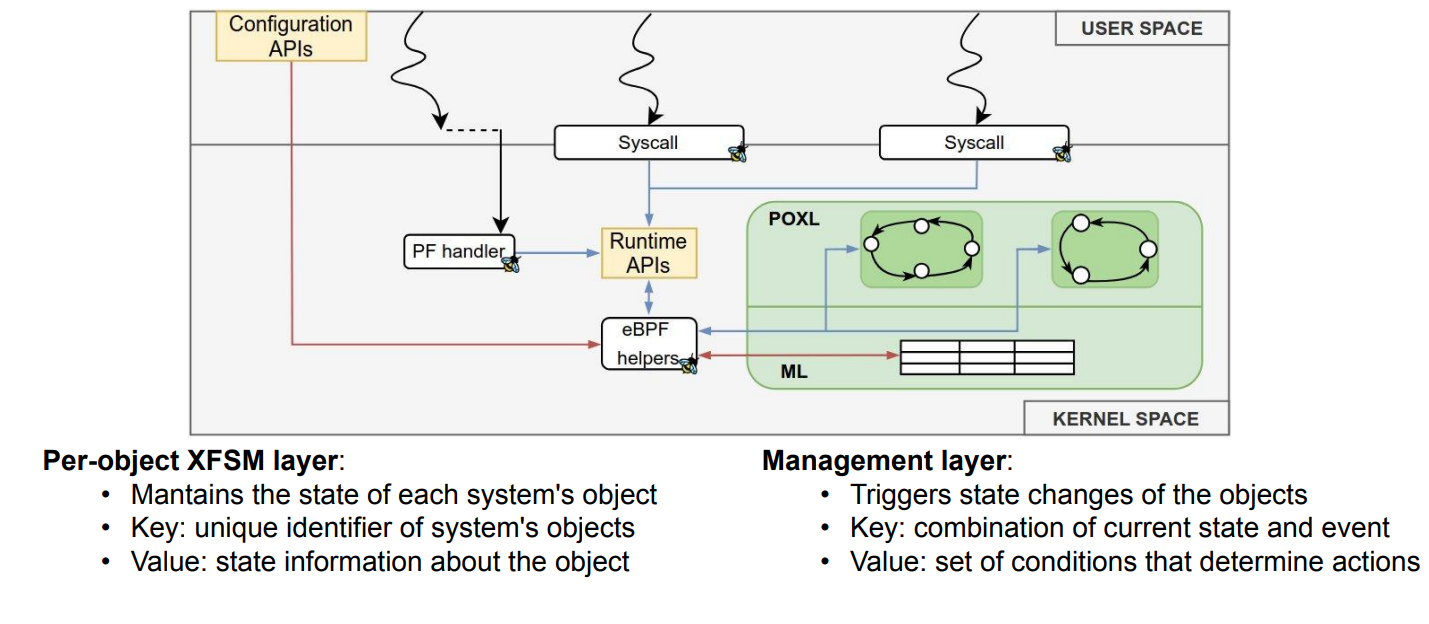
\includegraphics[width=0.8\textwidth]{immagini/SYS_08/architecture.png}
\caption{Architettura del monitoraggio stateful in Falco: gli eventi generati dalle system call vengono intercettati a livello kernel, trasferiti allo user space e arricchiti con informazioni di contesto (processo, utente, container). Il motore di regole analizza tali eventi mantenendo stato e correlazioni, evidenziando il compromesso tra profondità del monitoraggio, complessità di configurazione e overhead prestazionale.}
\end{figure}

Sebbene Falco fornisca una visibilità approfondita sul comportamento del sistema a runtime, il suo utilizzo in ambienti complessi richiede un’attenta configurazione. In contesti multi-tenant o altamente dinamici, un’eccessiva granularità delle regole può portare a un numero elevato di falsi positivi, rendendo difficile distinguere eventi realmente pericolosi da comportamenti legittimi.

In sistemi che generano milioni di system call al secondo, il monitoraggio continuo può introdurre un overhead non trascurabile. Per questo motivo è spesso necessario intervenire sul dimensionamento dei ring buffer, sul filtraggio degli eventi a livello kernel e sulla selezione mirata delle regole attive, bilanciando il livello di visibilità con l’impatto sulle prestazioni.

Un ulteriore aspetto critico riguarda la complessità operativa: la definizione di regole efficaci richiede una buona conoscenza del comportamento normale delle applicazioni monitorate. Regole troppo generiche possono risultare inefficaci, mentre regole troppo specifiche possono essere fragili e difficili da manutenere nel tempo.

Di conseguenza, Falco deve essere considerato come un componente di un ecosistema di sicurezza più ampio, da configurare e adattare in base al contesto operativo, piuttosto che come una soluzione universale applicabile senza tuning.
